\chapter{双拐点暴涨模型}

前面的章节中我们讨论了在超引力中构造拐点暴涨模型。接下来我们将简要介绍双拐点
暴涨模型以及在超引力框架内的实现,并针对该模型
计算了诱导引力波的能谱,发现该引力波信号有望在将来被空间引力波探测实验所发现。

% 双拐点暴涨模型
\section{超引力}

仍然考虑带有平移对称性的K\"ahler势\citep{ketov2016susy}
\begin{align}
    K=ic(\Phi-\bar\Phi)-\frac{1}{2}{(\Phi-\bar\Phi)}^2-\frac{\zeta}{4}{(\Phi-\bar\Phi)}^4,
\end{align}
其中$c$和$\zeta$为实参数。暴胀场取为手征超场$\Phi=(\phi+i\chi)/\sqrt{2}$的实部分量$\phi$。只要四次方项$\frac{\zeta}{4}{(\Phi-\bar\Phi)}^4$中的$\zeta$取得足够大,则暴胀场$\phi$在暴胀期间,场$\chi$的期望为$\langle\chi\rangle\approx0$。

参考了racetrack模型\citep{krasnikov1987supersymmetry,escoda2003saltatory,blanco2005racetrack}和其他模型\citep{ketov2016susy},我们选取如下形式的超势
\begin{align}
    W=a_0(1+a_1e^{-b_1\Phi}+a_2e^{-b_2\Phi}+a_3e^{-b_3\Phi}).
\end{align}

如果我们在宇宙学常数为零的真空中恢复来真空的超对称性(关于真空中的超对称破缺问题的讨论请参考文献\citep{gao2015inflection}),则F-term和势能V在$\Phi=0$处应当都为零,即$D_{\Phi}W=0$,$V=0$,这要求超势W满足约束条件
\begin{align}\label{eq:sp_constrain}
    W=\partial_{\Phi}W=0.
\end{align}
求解约束条件 (\ref{eq:sp_constrain}) 可以消去参数$a_1$和$a_2$
\begin{align}
    a_1\rightarrow \frac{b_2+a_3b_2-a_3b_3}{b_1-b_2},\qquad 
    a_2\rightarrow \frac{-b_1-a_3b_1+a_3b_3}{b_1-b_2}.
\end{align}
将K\"ahler势和超势代入到公式
\begin{align}
    V=e^{K/M^2_P}\lbrack
    D_{\Phi_i}W{(K^{-1})}^{ij^{\star}}D_{\Phi^{\star}_j}W^{\star}-3M^{-2}_P|W|^2\rbrack,
\end{align}
中,可以得到标量势能$V(\phi)$。其中,
\begin{align}
    D_{\Phi}W=\partial_{\Phi}W+M^{-2}_P{(\partial_{\Phi}K)}W,
\end{align}
以及K\"ahler度规的逆,
\begin{align}
    K^{ij\star} = \frac{\partial^2K}{\partial\Phi_i\partial\Phi^{\star}_j}.
\end{align}

当在参数空间中选取某组参数如
\begin{align}\label{eq:parameters}
    a_0 = 4.35\times 10^{-6},
    a_3 = 7\times 10^{-8},
    b_1 = 3.05,
    b_2 = 6.3868164,
    b_3 = -4.4,
    c = 2.8.
\end{align}
时,标量势能$V(\phi)$有两个近反射点,如图\ref{fig:potential}中所示。场取较大值处的拐点给出与当前CMB数据相一致的标量谱指标和张标比,较小值处的拐点可以使标量扰动的功率谱产生一个尖峰从而生成原初黑洞。
\begin{figure}[!htbp]
    \centering
    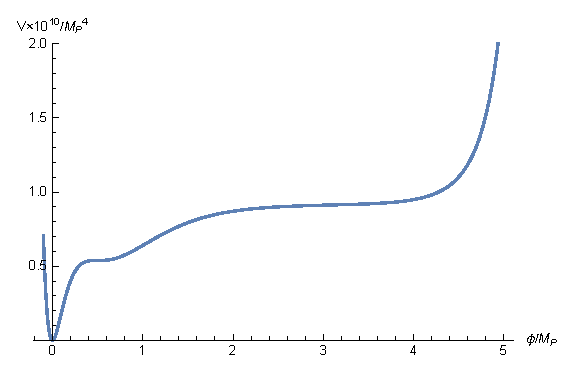
\includegraphics{Img/potential.eps}
    \caption{双拐点标量势能$V(\phi)$}\label{fig:potential}
\end{figure}

在FRW背景以及单场慢滚框架下,基于势能的慢滚参数$\epsilon_V$和$\eta_V$为
\begin{align}
    \epsilon_V &= \frac{M^2_P}{2}{\left(\frac{V\prime}{V}\right)}^2, \\
    \eta_V &= M^2_P {\left(\frac{V^{\prime\prime}}{V}\right)}.
\end{align}

由于在拐点附近势能变得极端平坦,因此慢滚近似不再适用\citep{dimopoulos2017ultra,germani2017primordial},代之以极端慢滚暴胀。此时为了更精确地求解暴胀过程,势能慢滚参数需要替换为哈勃慢滚参数\citep{schwarz2001higher,leach2002cosmological,schwarz2004primordial},
\begin{align}
    \epsilon_H &= -\frac{\dot{H}}{H^2}, \\
    \eta_H &= -\frac{\ddot{H}}{2H\dot{H}}=\epsilon_H-\frac{1}{2}\frac{d \ln\epsilon_H}{dN_e}, \\
    \xi_H &=
    \frac{\dddot{H}}{2H^2\dot{H}}-2\eta^2_H=\epsilon_H\eta_H-\frac{d\eta_H}{dN_e},
\end{align}

点$\dot{}$表示对宇宙时间$t$的导数,$N_e(t)$表示从视界穿过$k_{\star}$到暴胀结束期间的e-folding数,通常在取值在范围$50\sim60$之间。

标量谱指标及其跑动和张标比的领头阶可以用$\epsilon_H,\eta_H,\xi_H$来表示
\begin{align}
    n_s &= 1- 4\epsilon_H+2\eta_H, \\
    \alpha &= \frac{dn_s}{d\ln k}=10\epsilon_H\eta_H-8\epsilon_H^2-2\xi_H, \\
    r &= 16\epsilon_H.
\end{align}

在参数集 (\ref{eq:parameters}),相应的数值结果为
\begin{align}
    n_s = 0.9635,\qquad \alpha=-0.00369,\qquad r=0.00276,
\end{align}

当$k_{\star}=0.05Mpc^{-1}$时,在$68\%$的置信水平上与Planck
2018给出的对CMB的限制结果相一致\citep{akrami2018planck}
\begin{align}
    n_s = 0.9640\pm 0.0043,\qquad 
    \alpha = -0.0071\pm 0.0068,\qquad
    r < 0.079.
\end{align}

由于在拐点附近用近似表达式$\mathcal{P_R}\approx\frac{1}{8\pi^2M^2_P}\frac{H^2}{\epsilon_H}$计算得到的标量扰动会低于真实值\citep{gao2018primordial}。因此必须在模空间中数值求解MS方程,
\begin{align}\label{eq:ms}
    \frac{d^2u_k}{d\eta^2}+\left(k^2-\frac{1}{z}\frac{d^2z}{d\eta^2}\right)u_k=0,
\end{align}
其中$\eta$为共形时间,$z\equiv\frac{a}{\mathcal{H}}\frac{d\phi}{d\eta}$。初值条件取为Bunch-Davies真空\citep{bunch1978quantum}
\begin{align}
    u_k\rightarrow\frac{e^{-ik\eta}}{\sqrt{2k}},\quad\text{as}\quad
    \frac{k}{aH}\rightarrow\infty.
\end{align}

出于数值求解的方便,我们将共形时间$\eta$替换为$N_e$,把MS方程重写为\citep{ballesteros2018primordial}
\begin{align}
    \frac{d^2u_k}{dN^2_e}+\left(1-\epsilon_H\right)\frac{du_k}{dN_2}+
    \lbrack\frac{k^2}{\mathcal{H}^2}+\left(1+\epsilon_H-\eta_H\right)\left(\eta_H-2\right)-\frac{d\left(\epsilon_H-\eta_H\right)}{dN_e}=0,
\end{align}
原初功率谱由下式给出
\begin{align}
    \mathcal{P_R}=\frac{k^3}{2\pi^2}\lvert\frac{u_k}{z}\rvert^2_{k\ll
    \mathcal{H}}
\end{align}

图\ref{fig:pert}为MS方程\ref{eq:ms}基于参数集\ref{eq:parameters}的数值结果。从图中可以发现功率谱在小尺度有一个高峰,在CMB的尺度上大约增长了7个数量级。这样大的一个密度扰动使得原初黑洞能够通过引力塌缩形成。

\begin{figure}[!htbp]
    \centering
    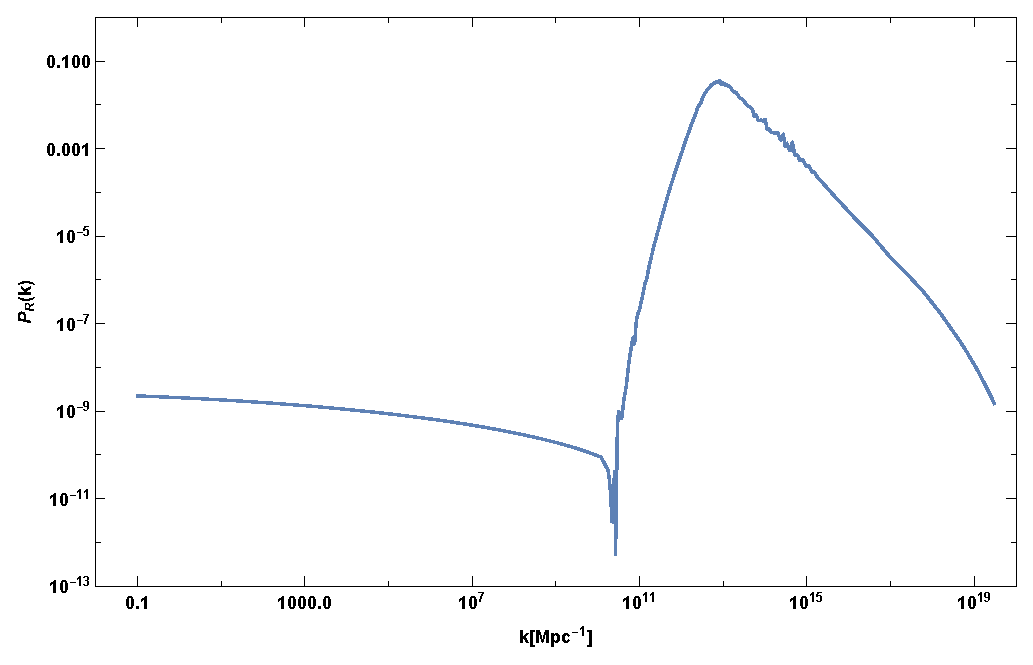
\includegraphics[width=4in]{Img/pert.eps}
    \caption{双拐点暴胀模型预测的标量扰动的原初功率谱$\mathcal{P_R}$}\label{fig:pert}
\end{figure}

% 双拐点暴涨模型在超引力中的实现
\section{在超引力中构造双拐点暴涨模型}
在第三章中曾提到在超引力中构造暴涨模型通常采用双场理论。通常我们期望暴涨过程中
演化方程只涉及暴涨场,因而要求其它的标量场稳定在使势函数取极值处。
在某些模型中,需要特别注意辅助场$S$在$s=0$处的稳定性。
有两种方法可以做到,一是在K\"ahler势中添加项$S\bar{S}$,二是选择不含标量自由度
的手征场$S$作为辅助场。后一种方法中涉及描述宇宙演化的只有一个无约束的手征超场$\Phi$场。
基于此,产生了一类无需引入额外非约束手征超场就能描述当前宇宙演化的暴涨模型
\citep{kallosh2015inflation,dall2014sgoldstino,linde2015does} 。


后来,Ketov和Terada提出了一类基于单手征超场$\Phi$的新暴涨理论
\citep{ketov2014generic,ketov2014inflation}。在 \citep{ketov2014generic}
中,提出了一种新的对数形式的K\"ahler势
\begin{equation}
  \label{eq:logarithmic-kahler-potential}
  K =
-3\ln \left[1+\frac{\Phi+\bar{\Phi}+\zeta{\left(\Phi+\bar{\Phi}\right)}^{4}}{\sqrt{3}}\right].
\end{equation}
$\zeta$是常系数。其中超场$\Phi$通常被分解为实部$\phi$和虚部$\chi$
\begin{equation}
  \Phi = \frac{1}{\sqrt{2}}(\phi+i\chi). 
\end{equation}
由于该K\"ahler势在平移变换$\Phi\rightarrow
\Phi+iC$下是不变的,超场$\Phi$的虚部$\chi$不会出现在K\"ahler势中,因此可以作为
暴涨场的候选者。在这个K\"ahler势中,四次方项的作用是在暴涨过程中将场$\phi$
稳定在零附近。并且K\"ahler势中并没有加入平方项和三次方项,尽管这些项不破坏对称
性,但是相应的系数可以通过调节超场$\Phi$和其它超场之间的耦合而压低。

不论超势取何种形式,当K\"ahler势取$(\ref{eq:logarithmic-kahler-potential})$式时,场$\Phi$的动能项系数为
\begin{equation}
  \label{eq:kinetic-coefficient-of-Phi}
  G(\phi,\chi) =
  \frac{3(1+32\zeta^2\phi^{6}-8\zeta\phi^2(3\sqrt{3}+\sqrt{2}\phi))}{{\left(\sqrt{3}+\sqrt{2}\phi+4\zeta\phi^{4}\right)}^2}.
\end{equation}

\begin{figure}[!http]
  \centering
  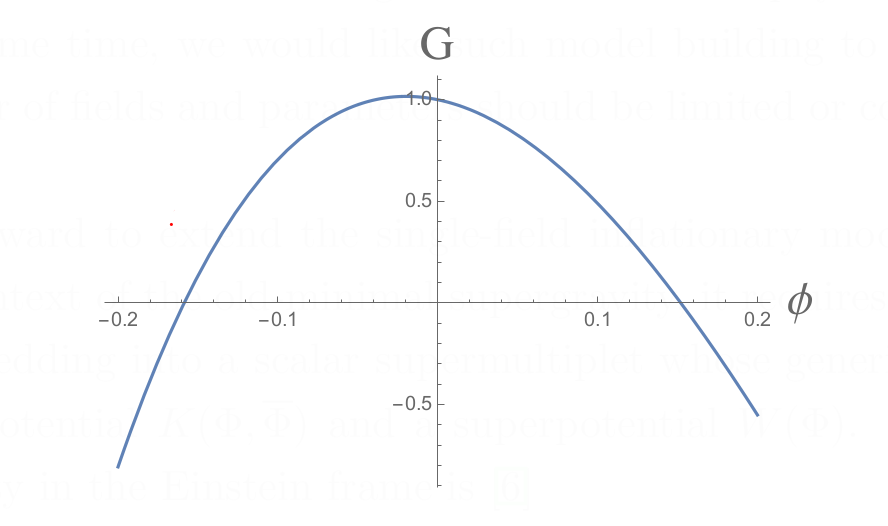
\includegraphics[width=5in]{Img/kinetic_coefficient_for_Phi.png}
  \caption{$\zeta=1$时,手征场$\Phi$的动能项系数与$\phi$的函数关系}\label{fig:kinetic-coefficient_for_Phi}
\end{figure}

从图$(\ref{fig:kinetic-coefficient_for_Phi})$可知,为了使$G>0$,$\phi$被限制在一
个有限的区间内。$\zeta$越大,$\phi$的取值区间越窄。因而在暴涨期间,标量场$\phi$的影响可以忽略,暴涨势近似为暴涨场$\chi$的函数,K\"ahler势中四次方项的调节作用
在这里清晰地体现出来了。当超势为
\begin{equation}
  W = \frac{1}{\sqrt{2}} f(-\sqrt{2}i\Phi),
\end{equation}
其中,$f$为实函数,沿暴涨场方向的暴涨势为
\begin{equation}
  V\simeq {\left[f_{,\chi}(\chi)\right]}^2.
\end{equation}
暴涨结束后,场朝着全局最小值滚去,最终得到一个超对称闵可夫斯基真空。这种情况对一
大类的超势都成立,同时也期望能在此基础上通过对K\"ahler势作一个微小的修正,能够抬升真空能得到德$\cdot$西特真空。然而no-go定理\citep{kallosh2014analytic}告诉我们对K\"ahler势和超势作一个无穷小修改,无法将具有超对称的闵可夫斯基真空连续地变化到德$\cdot$西特真空。举一个例子,当超势取如下形式时
\begin{equation}
  W=m(c\Phi+1),  
\end{equation}
\begin{figure}
  \centering
  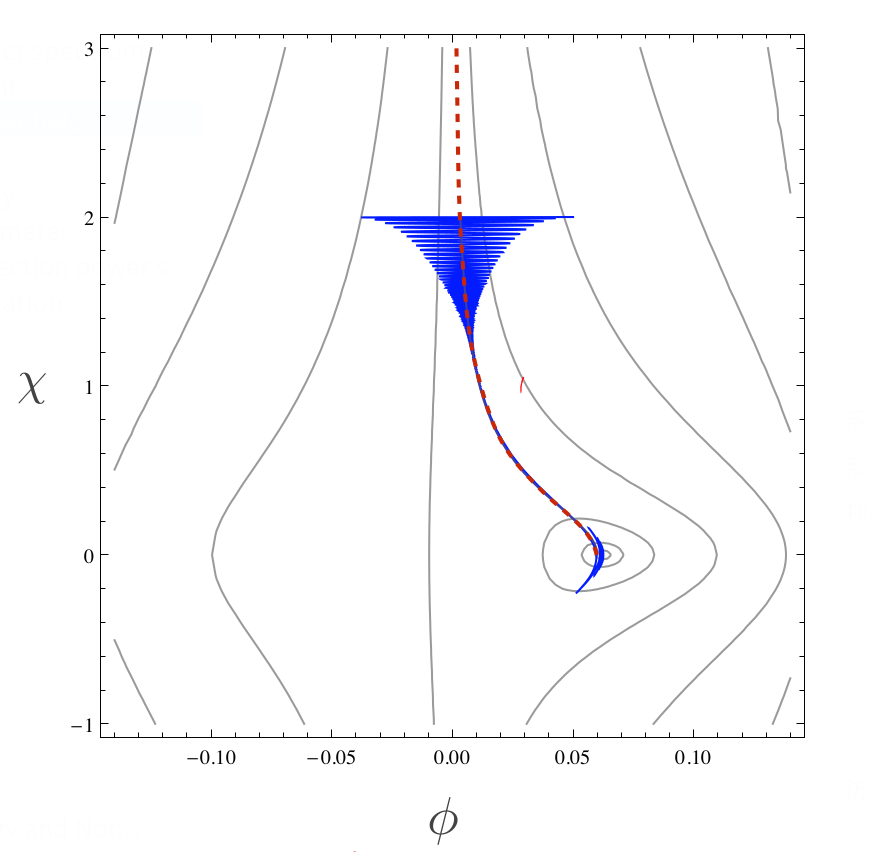
\includegraphics[width=5in]{Img/potential-for-linear-superpotential.png}
  \caption{蓝实线为数值计算得到的暴涨场的演化过程,红虚线为有效暴涨势的绝热近似。黑实线为暴涨势$V(\phi(\chi),
  \chi)$的对数等高线。当暴涨场靠近吸引子解前以及暴涨结束后都有一个震荡阶段。}\label{fig:potential-for-linear-superpotential}
\end{figure}
$c$和$d$为实参数,在$\phi=0$方向上暴涨势为
\begin{equation}
  V(\phi=0,\ \chi)=m^2c(c-2\sqrt{3}).
\end{equation}
显然参数$c$的大小将决定暴涨势大于零还是小于零。更具体的分析会发现,暴涨发生的过程并不完全在$\phi=0$方向。从图$(\ref{fig:potential-for-linear-superpotential})$中可以
看到,暴涨结束后得到的是一个超对称破缺的闵可夫斯基真空。通过对参数$c$进行微小的调节就能得到预期的德$\cdot$西特宇宙,$V_0\sim
10^{-120}$。但是代价为引起了强超对称破缺,得到的引力微子质量$m_{3/2}$比通常
理论预期的TeV量级高出多个量级。当考虑到粒子物理标准模型的时候,暴涨结束后是否
恢复超对称性是一件很重要的事情。例如
\citep{endo2006moduli,nakamura2006gravitino,kawasaki2006gravitino,kawasaki2006gravitino-overproduction,asaka2006gravitinos}
指出当真空超对称性破缺时,早期宇宙中从暴涨场衰变得到的引力微子数目会增多,
而这将引起灾难。另外\citep{degrassi2012higgs}中指出如果超对称破缺的能标过高,
电弱真空会遇到稳定性问题。

为了规避上述困难,同时在不破坏no-go定理的前提下,有两种方法既能抬升真空势能
得到德$\cdot$西特真空又能避免大的超对称破缺。一是引入额外的手征多态
(Polonyi场),并且对其施加强约束尽可能降低其对宇宙演化的影响
\citep{dudas2013strong}。另一个方法是引入零幂手征超场
\citep{ferrara2014cosmology,kallosh2015inflation,dall2014sgoldstino,kallosh2015inflation-de-sitter,linde2015does},
并且能从弦论中找到理论解释\citep{kallosh2014emergence}。

沿着这个思路,\citep{ketov2016susy}讨论了暴涨结束后恢复超对称性的条件,以及通过添加一个满足零幂条件$S^2=0$的Polonyi超场作为超对称破缺场$S$来控制超对称破缺的能标。


仍然考虑带有平移对称性的K\"ahler势\citep{ketov2016susy}
\begin{align}
    K=ic(\Phi-\bar\Phi)-\frac{1}{2}{(\Phi-\bar\Phi)}^2-\frac{\zeta}{4}{(\Phi-\bar\Phi)}^4,
\end{align}
其中$c$和$\zeta$为实参数。暴涨场取为手征超场$\Phi=(\phi+i\chi)/\sqrt{2}$的实部分量$\phi$。只要四次方项$\frac{\zeta}{4}{(\Phi-\bar\Phi)}^4$中的$\zeta$取得足够大,则暴涨场$\phi$在暴涨期间,场$\chi$的期望为$\langle\chi\rangle\approx0$。

参考了racetrack模型\citep{krasnikov1987supersymmetry,escoda2003saltatory,blanco2005racetrack}和其他模型\citep{ketov2016susy},我们选取如下形式的超势
\begin{align}
    W=a_0(1+a_1e^{-b_1\Phi}+a_2e^{-b_2\Phi}+a_3e^{-b_3\Phi}).
\end{align}

如果我们在宇宙学常数为零的真空中恢复了真空的超对称性
(关于真空中的超对称破缺问题的讨论请参考文献
\citep{gao2015inflection}),则F-term和暴涨势V在$\Phi=0$处应当都为零,
即$D_{\Phi}W=0$,$V=0$,这要求超势W满足约束条件
\begin{align}\label{eq:sp_constrain}
    W=\partial_{\Phi}W=0.
\end{align}
求解约束条件 (\ref{eq:sp_constrain}) 可以消去参数$a_1$和$a_2$
\begin{align}
    a_1\rightarrow \frac{b_2+a_3b_2-a_3b_3}{b_1-b_2},\qquad 
    a_2\rightarrow \frac{-b_1-a_3b_1+a_3b_3}{b_1-b_2}.
\end{align}
将K\"ahler势和超势代入到公式
\begin{align}
    V=e^{K}\lbrack
    D_{\Phi_i}W{(K^{-1})}^{ij^{*}}D_{\Phi^{*}_j}W^{*} - 3|W|^2\rbrack,
\end{align}
中,可以得到标量势$V(\phi)$。其中,
\begin{align}
    D_{\Phi}W=\partial_{\Phi}W + {(\partial_{\Phi}K)}W.
\end{align}
以及K\"ahler度规的逆,
\begin{align}
    K^{ij*} = \frac{\partial^2K}{\partial\Phi_i\partial\Phi^{*}_j}.
\end{align}

当在参数空间中选取某组参数如
\begin{align}\label{eq:parameters}
    a_0 = 4.35\times 10^{-6},
    a_3 = 7\times 10^{-8},
    b_1 = 3.05,
    b_2 = 6.3868164,
    b_3 = -4.4,
    c = 2.8.
\end{align}
时,标量势$V(\phi)$有两个近反射点,如图\ref{fig:potential}中所示。
场取较大值处的拐点给出与当前CMB数据相一致的标量功率谱的谱指标和张标比,
较小值处的拐点可以使标量扰动的功率谱产生一个尖峰从而生成原初黑洞。
\begin{figure}[!htbp]
    \centering
    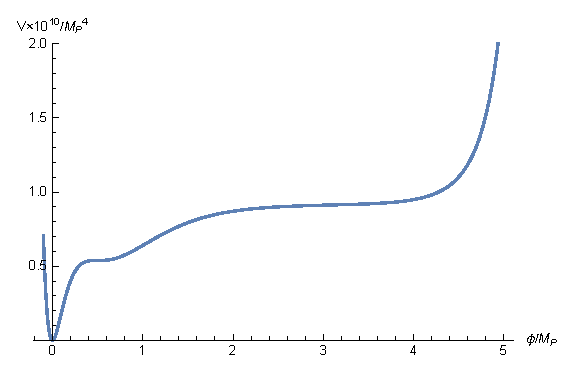
\includegraphics[width=5in]{Img/potential.eps}
    \caption{双拐点标量势$V(\phi)$}\label{fig:potential}
\end{figure}

在FLRW背景以及单场慢滚框架下,基于势能的慢滚参数$\epsilon_V$和$\eta_V$为
\begin{align}
  \epsilon_V &= \frac{1}{2}{\left(\frac{V_{,\phi}}{V(\phi)}\right)}^2, \\
  \eta_V &= \frac{V_{,\phi \phi}}{V(\phi)}.
\end{align}

由于在拐点附近暴涨势变得极端平坦,因此慢滚近似不再适用\citep{dimopoulos2017ultra,germani2017primordial},代之以极端慢滚暴涨。此时为了更精确地求解暴涨过程,势能慢滚参数需要替换为哈勃慢滚参数\citep{schwarz2001higher,leach2002cosmological,schwarz2004primordial},
\begin{align}
    \epsilon_H &= -\frac{\dot{H}}{H^2}, \\
    \eta_H &= -\frac{\ddot{H}}{2H\dot{H}}=\epsilon_H-\frac{1}{2}\frac{d \ln\epsilon_H}{dN_e}, \\
    \xi_H &=
    \frac{\dddot{H}}{2H^2\dot{H}}-2\eta^2_H=\epsilon_H\eta_H-\frac{d\eta_H}{dN_e},
\end{align}
其中,$N_e(t)$表示从视界穿过$k_{\star}$到暴涨结束期间的e-folding数,通常在取值在范围$50\sim60$之间。

标量扰动谱指标及其跑动和张标比的领头阶可以用$\epsilon_H,\eta_H,\xi_H$来表示
\begin{align}
    n_s &= 1- 4\epsilon_H+2\eta_H, \\
    \alpha &= \frac{dn_s}{d\ln k}=10\epsilon_H\eta_H-8\epsilon_H^2-2\xi_H, \\
    r &= 16\epsilon_H.
\end{align}

在参数集 (\ref{eq:parameters})下,相应的数值结果为
\begin{align}
  n_s &= 0.9635,\\
  \alpha&=-0.00369,\\
  r&=0.00276,
\end{align}

当$k_{\star}=0.05Mpc^{-1}$时,在$68\%$的置信水平上与Planck
2018给出的对CMB的限制结果相一致\citep{akrami2018planck}
\begin{align}
  n_s &= 0.9640\pm 0.0043,\\
  \alpha &= -0.0071\pm 0.0068,\\
  r &< 0.079.
\end{align}

标量扰动的功率谱在慢滚暴涨模型通常用近似公式
\begin{equation}
  \label{eq:scalar-perturbation-power-spectrum}
  \mathcal{P}_{\mathcal{R}} = \frac{V}{24\pi^2 \epsilon_V}.
\end{equation}
计算得到。由于在拐点处,暴涨势导数为零,因此使用势能慢滚参数的功率谱近似公式在
拐点处产生无穷大,导致公式失效。因而
\citep{germani2017primordial,motohashi2017primordial}中采用了不同的近似公式,
由于哈勃慢滚参数在整个暴涨期间始终大于零,因此基于哈勃慢滚参数的近似功率谱公式
\begin{equation}
  \label{eq:scalar-perturbation-power-spectrum-hubble}
  \mathcal{P}_{\mathcal{R}} \simeq
  \frac{1}{8\pi^2}\frac{H^2}{\epsilon_H}.
\end{equation}
将会给出更准确的结果。不过仍然指出这种近似可能会导致对PBH的质量函数产生错误的
估计,因而 \citep{ballesteros2018primordial}中根据Mukhanov-Sasaki (MS)公式
\citep{sasaki1986large,mukhanov1988quantum}数值求解精确的功率谱。 
Mukhanov-Sasaki (MS)方程为
\begin{align}\label{eq:ms}
    \frac{d^2u_k}{d\eta^2}+\left(k^2-\frac{1}{z}\frac{d^2z}{d\eta^2}\right)u_k=0,
\end{align}
其中$\eta$为共形时间,$z\equiv\frac{a}{\mathcal{H}}\frac{d\phi}{d\eta}$。初值条件取为Bunch-Davies真空\citep{bunch1978quantum}
\begin{align}
    u_k\rightarrow\frac{e^{-ik\eta}}{\sqrt{2k}},\quad\text{as}\quad
    \frac{k}{aH}\rightarrow\infty.
\end{align}

出于数值求解的方便,我们将共形时间$\eta$替换为$N_e$,把MS方程重写为\citep{ballesteros2018primordial}
\begin{align}
    \frac{d^2u_k}{dN^2_e}+\left(1-\epsilon_H\right)\frac{du_k}{dN_2}+
    \lbrack\frac{k^2}{\mathcal{H}^2}+\left(1+\epsilon_H-\eta_H\right)\left(\eta_H-2\right)-\frac{d\left(\epsilon_H-\eta_H\right)}{dN_e}=0,
\end{align}
原初功率谱由下式给出
\begin{align}
    \mathcal{P_R}=\frac{k^3}{2\pi^2}\left\lvert\frac{u_k}{z}\right\rvert^2_{k\ll
    \mathcal{H}}.
\end{align}

图\ref{fig:pert}为MS方程\ref{eq:ms}基于参数集\ref{eq:parameters}的数值结果。从图中可以发现功率谱在小尺度有一个高峰,在CMB的尺度上大约增长了7个数量级。这样大的一个密度扰动使得原初黑洞能够通过引力塌缩形成。

\begin{figure}[!htbp]
    \centering
    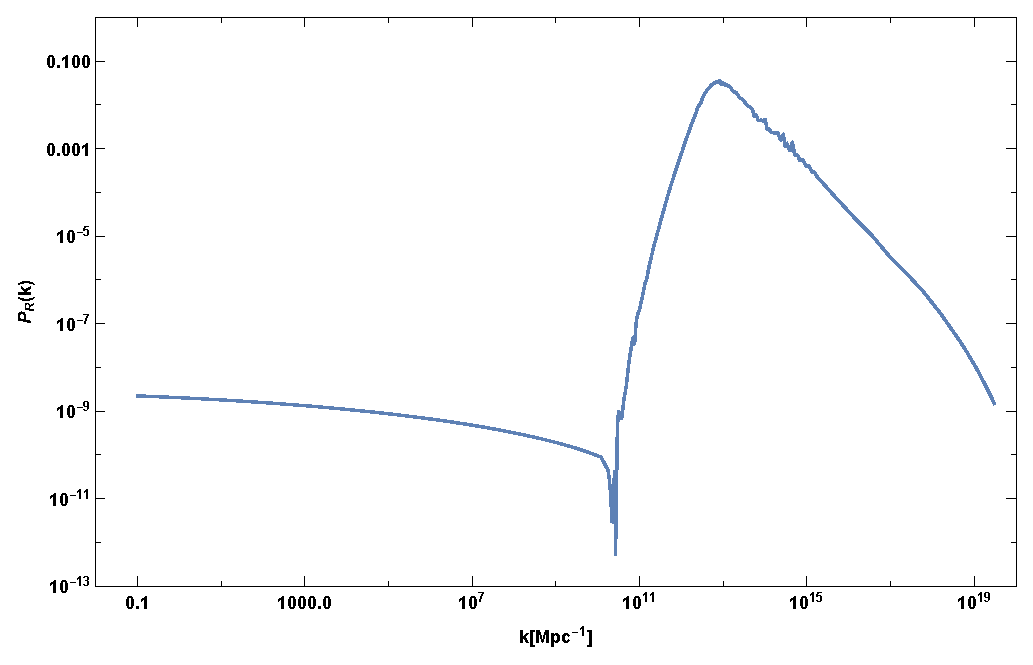
\includegraphics[width=5in]{Img/pert.eps}
    \caption{双拐点暴涨模型预测的标量扰动的原初功率谱$\mathcal{P_R}$}\label{fig:pert}
\end{figure}

% 原初黑洞——不用
% \section{原初黑洞}
当某个原初密度扰动足够大的尺度在暴涨结束后重新进入视界时,由引力塌缩可能形成原初黑洞。
一般黑洞的质量$M$正比于当时的一个哈勃体积内的总质量$M_H$,比例系数为$\gamma$。
\begin{equation}
    M = \gamma M_H = \gamma \frac{4}{3}\pi\rho H^{-3}
\end{equation}
系数$\gamma$取决于引力塌缩的过程,与采取的模型有关,一般取
$0.2$在辐射为主时期\citep{carr1975primordial}。利用熵守恒$d(g_s(T)T^3a^3)/dt=0$和$\rho\propto
g(T)T^4$,可以得到辐射为主时期:
\begin{equation}
    \label{eq:mass_pbh}
    M=\gamma M_{H(eq)}{\left(\frac{g(T_f)}{g(T_{eq})}\right)}^{1/2}
    {\left(\frac{g_s(T_f)}{g_s(T_{eq})}\right)}^{-2/3}
    {\left(\frac{k}{k_{eq}}\right)}^{-2}
\end{equation}

$M_{H(eq)}$表示辐射-物质相等时的视界内的总质量。因为物质为主时期
$H^2\propto \rho \propto a^{-3}$和 $k=aH$,故有
\begin{align*}
    \label{eq:horizon_mass_eq}
    M_{H(eq)} &= \frac{4}{3}\pi\rho_{eq}H_{eq}^{-3} \\
    &= \frac{4}{3}\pi\rho_m
    a_{eq}^{-3}{\left(\frac{k_{eq}}{a_{eq}}\right)}^{-3}\\
    &= \frac{4}{3}\pi \Omega_m \rho_{0,crit}k^{-3}_{eq} \\
    &\approx 3\times 10^{50}\ g
\end{align*}

在辐射为主时期假设 $g(T)=g_s(T)$
是一个好的近似,以及最新Planck
2018数据\citep{aghanim2018planck}给出的$k_{eq}=0.073\Omega_m
h^2\ \text{Mpc}^{-1}$。于是{(\ref{eq:mass_pbh})}可写成
\begin{equation}
    M(k) =
    10^{18}g\left(\frac{\gamma}{0.2}\right){\left(\frac{g(T_f)}{106.75}\right)}^{-1/6}
    {\left(\frac{k}{7\times10^{13}\ \text{Mpc}^{-1}}\right)}^{-2}
\end{equation}
$M(k)$表示共动波数$k$重新进入视界时形成的黑洞的质量。

在Press-schechter引力塌缩模型中\citep{press1974formation},质量M的原初黑洞的生成率由一个高斯随机概率分布决定。当相对密度扰动$\delta$大于某个阈值$\delta_c$时,视界内的物质将在引力的作用下塌缩形成一个黑洞,那么质量为M的原初黑洞所占丰度$\beta(M)$将由高斯分布的分布函数给出:
\begin{align}
    \label{eq:mass_fraction_pbh}
    \beta(M) = \frac{1}{\sqrt{2\pi \sigma^2(M)}}\int_{\delta_c}^{\infty}
    d\delta\ \text{exp}\left(\frac{-\delta^2}{2\sigma^2(M)}\right).
\end{align}

唯一不确定的还剩下方差$\sigma^2(M)$。对它的计算一般采用如下方式,将空间粗粒化成一个个尺度为$R=1/k$的区域,并用高斯窗口函数$W(x)=\text{exp}(-x^2/2)$将相对密度扰动光滑化,最后对所有区域求$\delta$的方差作为$\sigma^2(M)$:
\begin{align}
    \sigma^2(M(k)) &= \int \frac{dq}{q}W{(qR)}^2 \\
    &= \frac{16}{81}\int \frac{dq}{q} {(qR)}^4 \mathcal{P_R}(q)W{(qR)}^2,
\end{align}

对应$k$模的原初黑洞对暗物质的贡献为
\begin{align*}
    f_{PBH}(M) &\equiv \frac{\Omega_{PBH}(M)}{\Omega_c} =
    \frac{\rho_{PBH}(M)}{\rho_m}\mid_{eq}\frac{\Omega_m h^2}{\Omega_c h^2}
    \\
    &= \frac{\beta(M)}{8\times
    10^{-16}}{\left(\frac{\gamma}{0.2}\right)}^{3/2}{\left(\frac{g(T_M)}{106.75}\right)}^{-1/4}{\left(\frac{M}{10^{18}\ g}\right)}^{-1/2}
\end{align*}

其中暗物质的丰度取为$\Omega_c h^2 \simeq 0.12$\citep{aghanim2018planck}。当前所有原初黑洞的丰度由积分式给出;
\begin{align}
    \label{eq:abundence_pbh}
    \Omega_{PBH} = \int \frac{dM}{M}\Omega_{PBH}(M),
\end{align}

公式{(\ref{eq:mass_fraction_pbh})}说明原初黑洞的质量分数对临界塌缩密度$\delta_c$非常敏感。在辐射为主时期,近期多数在这方面的研究文章\citep{musco2005computations,musco2009primordial,musco2013primordial,harada2013threshold}建议$\delta_c$取值大约为$0.45$。此时若希望原初黑洞能在$\mathcal{O}(1)$量级成为暗物质组成成分,那么曲率扰动的原初功率谱需要增大到大约为$\mathcal{P_R}\simeq
10^{-2}$。而在CMB尺度上,扰动大约为$\mathcal{P_R}\simeq
10^{-9}$。因此我们需要一个机制,使得对应某个尺度范围(相应的某个原初黑洞的质量区间)的曲率扰动在离开视界时产生一个峰。

把原初黑洞的质量和e-folding数联系起来,能使我们对其形成于哪个时期有一个相对清晰的概念。为了做到这一点,需要假设在暴涨时期,哈勃“常数”近似为常数。所以$k$模离开视界时相对于某个基准$k_\star$已经膨胀了大约
\begin{align}
    \label{eq:delta_efolding}
    \Delta N^{\star}_e = \log \frac{a_k}{a_\star} = \log\frac{a_k
    H_I}{k_\star} = \log \frac{a_f H_f}{k_\star},
\end{align}
仍然假设对应熵和能量密度的有效自由度数相等,于是可以得到公式\citep{motohashi2017primordial}:
\begin{align}
    \Delta N^{\star}_e =
    -\frac{1}{2}\log\frac{M}{M_\odot}+\frac{1}{2}\log\gamma
    +\frac{1}{12}\log\frac{g(T)}{106.75}+\frac{1}{2}\log\frac{4.4\times10^{24}\Omega_r
    H^2_0}{k^2_{\star}}, 
\end{align}
其中辐射密度为$\Omega_r h^2=4.18\times10^{-5}$,哈勃常数为$H_0\simeq
0.0007\text{Mpc}^{-1}$。若选择基准为$k_\star =
  0.05\text{Mpc}^{-1}$,参考Planck组的数据,上式可以变为
\begin{align}
    \Delta N^{\star}_e = 18.37-\frac{1}{2}\log\frac{M}{M_\odot}.
\end{align}



% 诱导引力波
\section{引力波}


% 小结
\section{小结}

在双拐点暴涨模型,
其中一个拐点产生与CMB观测一致的功率谱,另一个拐点使原初功率谱在小尺度上产生一个峰值
,这个峰不仅能使扰动在辐射为主时期重新进入视界时产生原初黑洞,同时也能让诱导
引力波的信号在该尺度附近得到增强。由于在拐点附近暴涨势极端平坦,因而通常的慢滚近似
不再适用,只能通过数值算法得到曲率扰动的功率谱。另一方面,我们在共形牛顿规范下
求得诱导引力波满足的演化方程,并且得到了诱导引力波的功率谱$\mathcal{P}_{h}$和曲率扰动的
功率谱$\mathcal{P}_{\mathcal{R}}$的关系,最终获得了诱导引力波能谱的表达式。
进行计算之后,发现诱导引力波的信号存在一个峰,且峰的高度在LISA与Taiji的期望
灵敏度曲线之上,意味着模型预言的诱导引力波信号有望被LISA和Taiji的实验观测到。

